\chapter{Systematic Uncertainties}

The nominal simulated shape of the \Nb distribution is allowed to vary by the inclusion of systematic uncertainties.
Each uncertainty is incorporated in the fit with template \Nb histograms to account for the effects of the systematic variation and a nuisance parameter $\theta$ to control the variation amplitude.
The nuisance parameters are subject to Gaussian constraints, normalized so that $\theta=0$ corresponds to the nominal \Nb shape and $\theta=\pm1$ corresponds to $\pm1$ standard deviation (s.d.)\ variation of the systematic uncertainty.
These uncertainties affect only the \Nb shape for \ttbar, QCD, and W+jets backgrounds, because their normalizations are determined from data, while for the other (subleading) backgrounds the uncertainties affect both the \Nb shape and normalization.

\begin{section}{Gluon Splitting}

The primary source of systematic uncertainty is on the modelling of the rate of gluon splitting, as events with a gluon splitting to \bbbar provide an additional source of b quarks in events.
As this process may not be properly simulated, constraining the splitting rate in data is crucial for establishing a robust prediction of the \Nb distribution.
The dominant contribution of this effect is due to gluons that split specifically to b~quark pairs, so the phrase ``gluon splitting'' will hereafter refer exclusively to gluon splitting to \bbbar.
One way to select a data sample enriched in gluon splitting events is to use the \dRbb distribution, where \dRbb is defined as the $\Delta R$ between two b-tagged jets, as pairs of b-tagged jets resulting from the same gluon splitting tend to have smaller values of \dRbb than pairs resulting from hard scatter b-quarks or fakes.
This can be seen in Figure~\ref{fig:dRbb_shapes}, which shows the dRbb distribution in simulated QCD events with $\Nb = 2$ for three important categories:
Events that have a correlated pair of b-tagged jets originating from a gluon splitting (green, denoted GSbb) populate the low-\dRbb region, while events without gluon splitting (yellow, denoted noGS) or where the splitting yields zero one b-tagged jets (blue, denoted GSb) populate the low-and high-\dRbb regions roughly equally.

\begin{figure}[tbp!]
\begin{center}
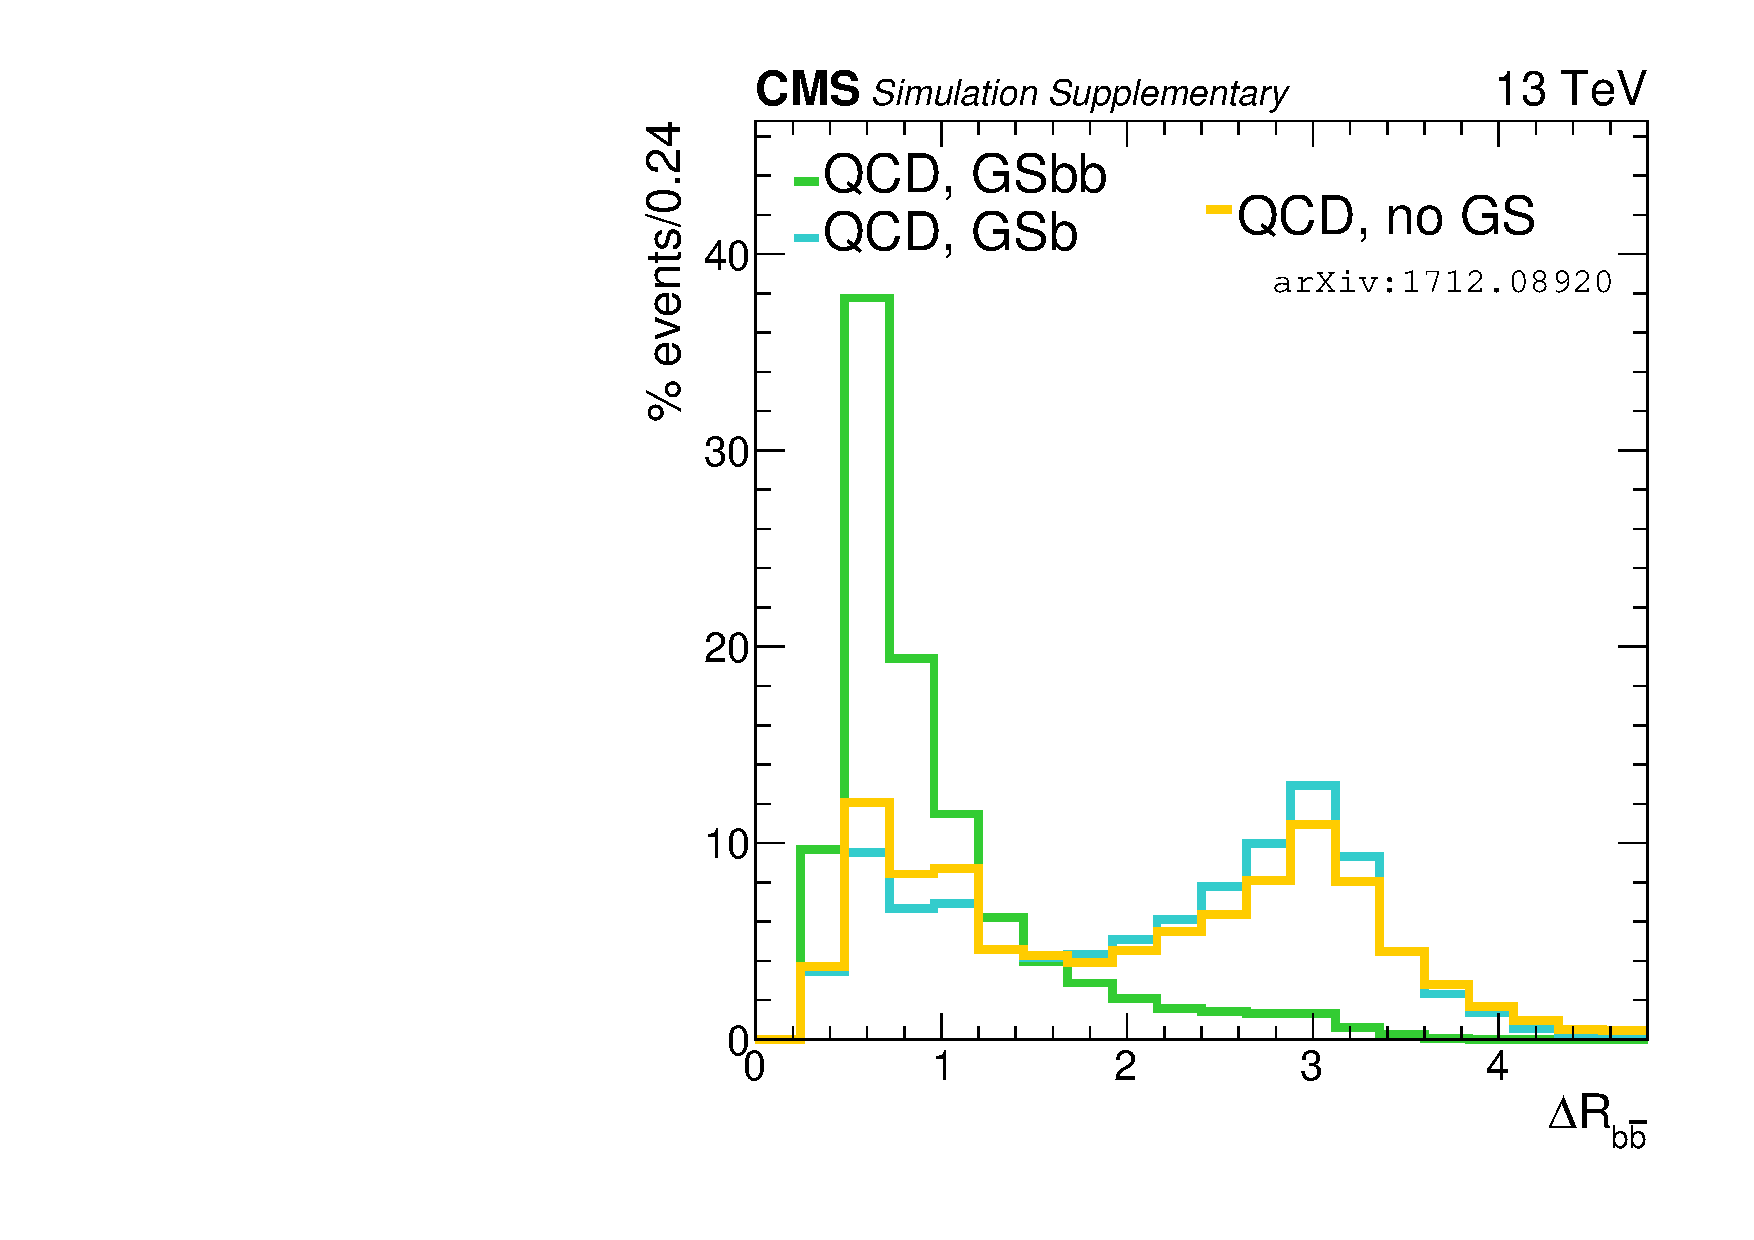
\includegraphics[angle=0,width=0.60\columnwidth]{fig/dRbb_shapes.pdf}
\end{center}
\caption{The \dRbb distribution shapes for the three gluon splitting categories: 
Events with a pair of b-tagged jets resulting from gluon splitting (green), events with a gluon splitting yielding fewer than 2 b-tagged jets (blue), and events without a gluon splitting to \bbbar.
These events are selected by requiring $\Nleps = 0$, $\HT > 1500~\GeV$, $\MJ > 500~\GeV$, $\Njets \geq 4$, and $\Nb = 2$.}
\label{fig:dRbb_shapes}
\end{figure}

Gluon splittings can contribute less than 2 b-tagged jets either because the quarks are collimated into a single jet, one of the b-tagged jets is not tagged, or because one of the jets fails to pass the jet selection criteria, typically because it is too soft.
The relative fractions of these contributions is shown in Figure~\ref{fig:gs_categories}.

\begin{figure}[tbp!]
\begin{center}
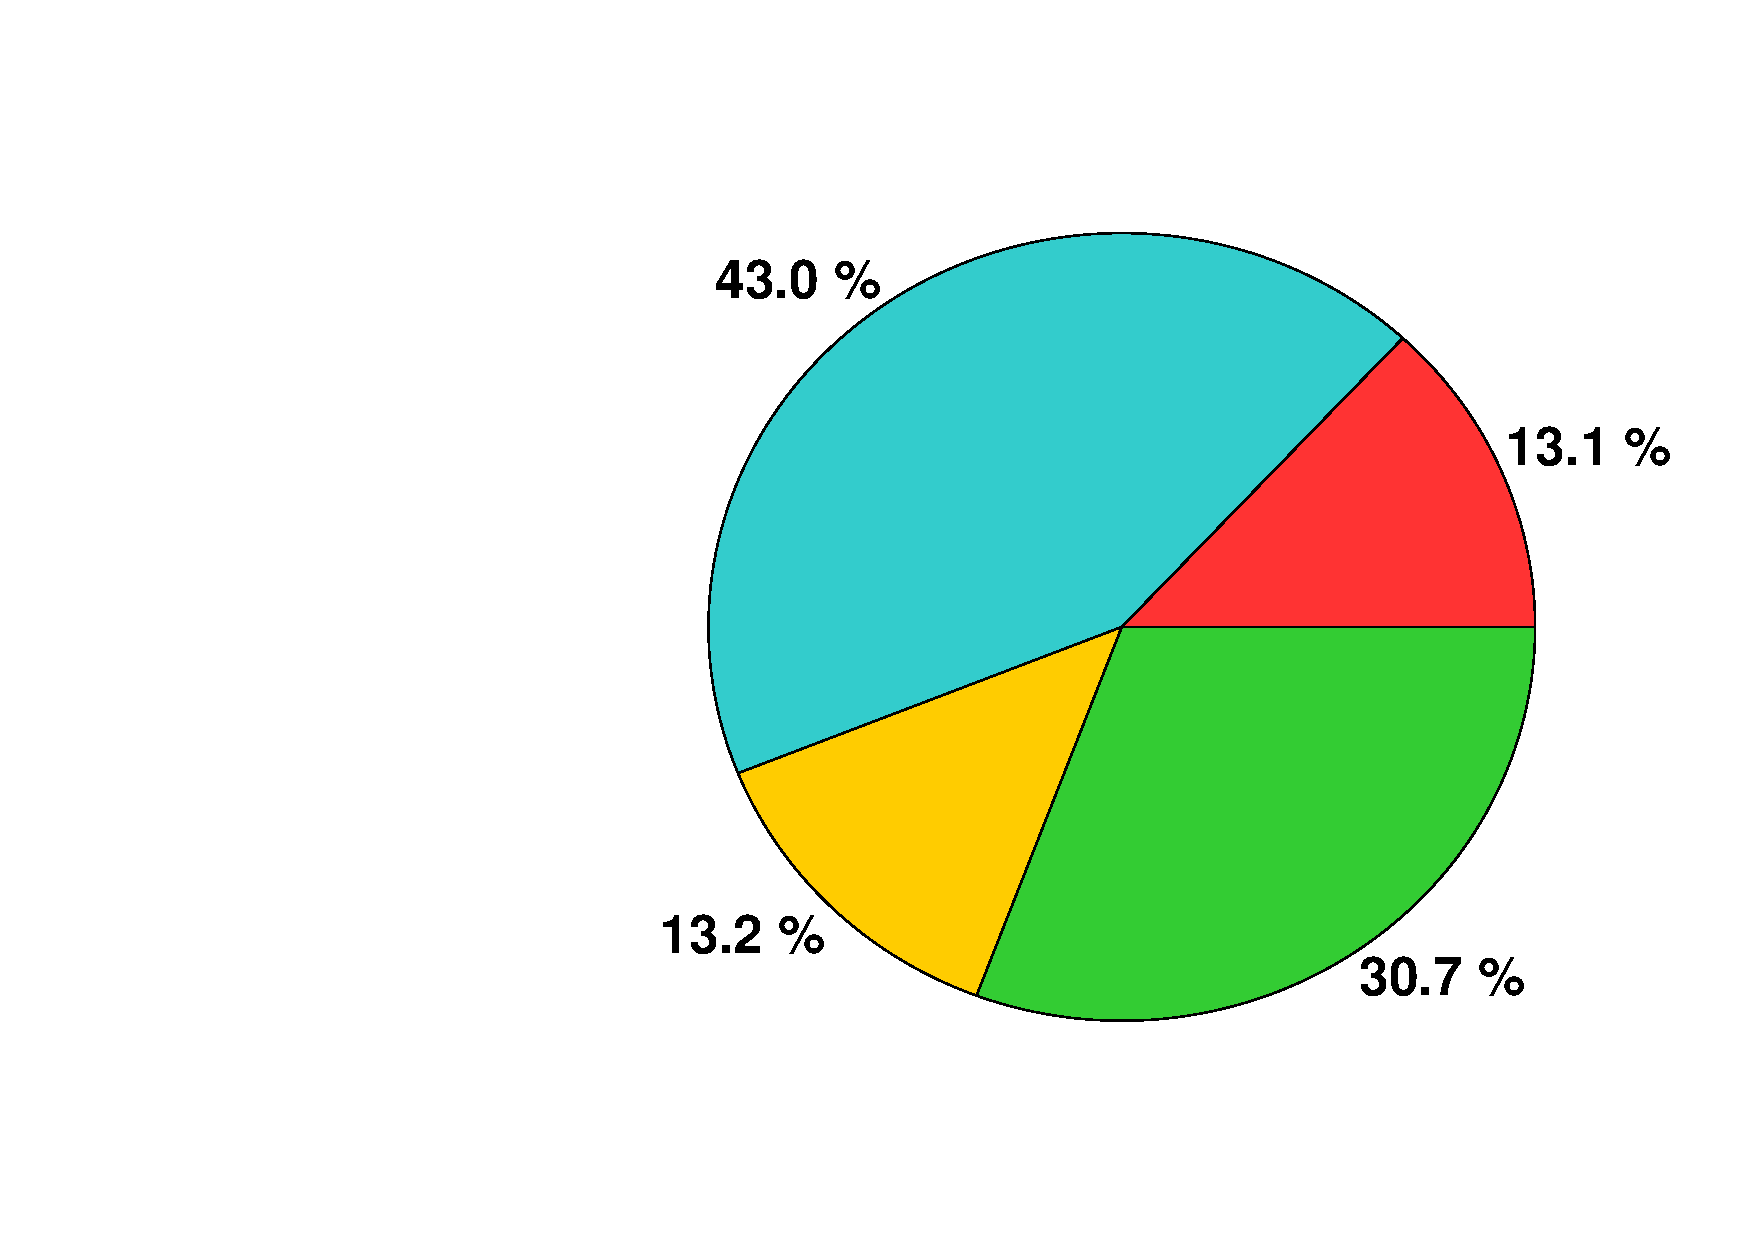
\includegraphics[angle=0,width=0.45\columnwidth]{fig/gs_piechart.pdf}
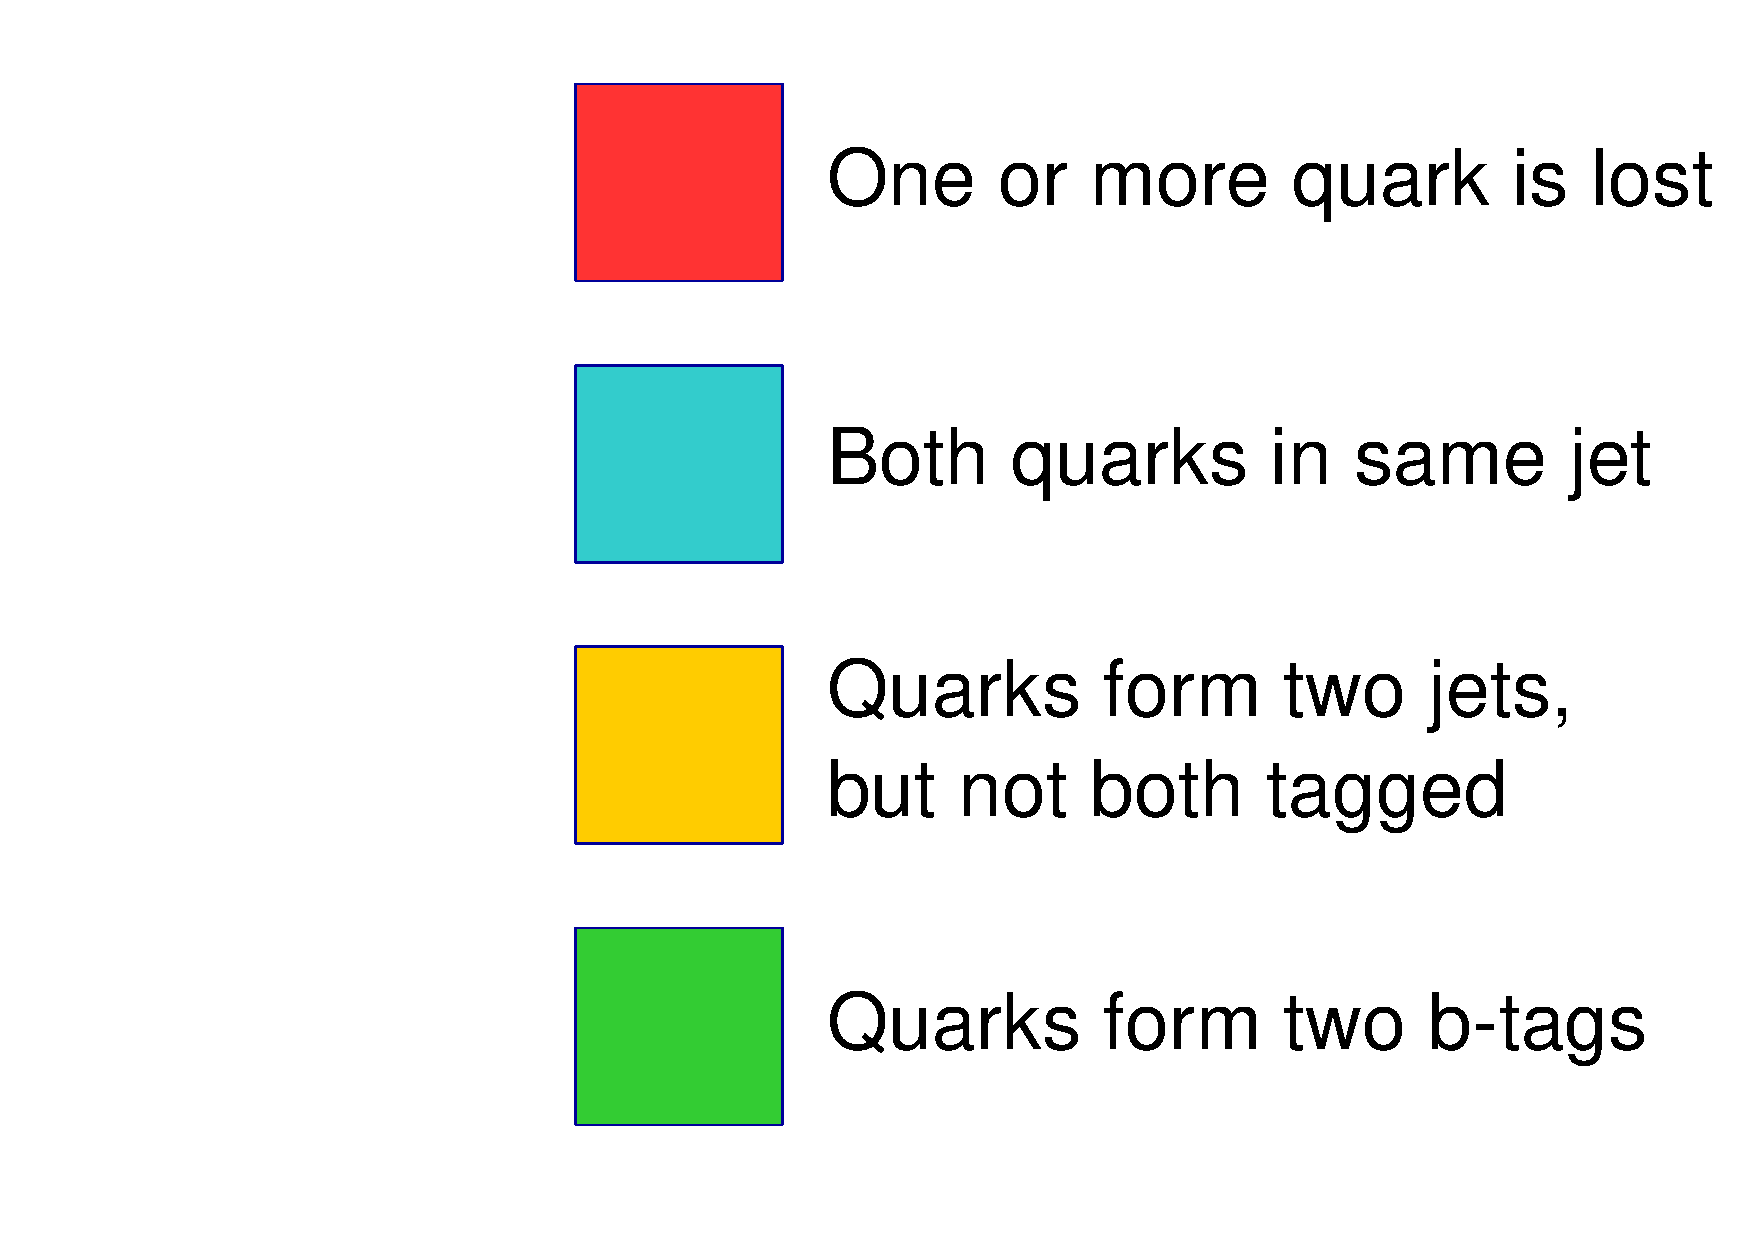
\includegraphics[angle=0,width=0.45\columnwidth]{fig/gs_piechart_legend.pdf}
\end{center}
\caption{The relative fraction of the possible final states that occur from gluon splitting to \bbbar for events satisfying $\Nleps = 0$, $\HT > 1500~\GeV$, $\MJ > 500~\GeV$, $\Njets \geq 4$, and $\Nb = 2$.}
\label{fig:gs_categories}
\end{figure}

The gluon splitting rate is the constrained by fitting the \dRbb distribution by using the difference in shapes of the GSbb, GSb, and noGS categories.
This fit varies the normalization of the GSbb and GSb (varied together) and the noGS contributions in order to extract the relative contributions of events with and without a gluon splitting.
It is performed in four equal bins in the range of $0 \leq \dRbb < 4.8$ with events selected by requiring $\Nleps = 0$, $\HT > 1500\GeV$, $\Nb = 2$, $\Njets \geq 4$, and $\MJ > 500~\GeV$ as the gluon splitting signal in a $\Nleps = 1$ control sample is contaminated by b~quarks from the decay of top quarks.
Additionally, the $\Nleps = 0$ control sample is formed from a subset of the data that is selected to be most stable in the b~tagging algorithm performance, since the precision of the \dRbb fit is not limited by the data sample size.
This choice isolates the physical effects of gluon splitting from the potential time dependence of the b~tagging performance due to variations in experimental conditions, which are separately incorporated by the b-tag scale factor uncertainties.
% WHY NLEPS=0 region also works for NLEPS=1

The \dRbb fit extracts a weight of $0.77 \pm 0.09$ for gluon splitting events and a weight of $1.21 \pm 0.08$ for non-gluon splitting events.
The post-fit distributions are shown in Figure~\ref{fig:gs_fitresult}.
The GSbb and GSb categories are plotted separately to demonstrate the difference in shapes.
The discrepancy in the last bin does not significantly impact the fit because the higher yield bins at lower values of \dRbb constrain the fit.
The deviations of these weights from unity, summed in quadrature with their post-fit uncertainty, are used to form the $\pm 1$~s.d.\ variations of the gluon splitting rate nuisance parameter by applying weights of $1 \pm 0.25$ to gluon splitting events and $1 \mp 0.22$ to non-gluon splitting events in an anti-correlated manner.
The fit results are used as a measure of the uncertainty on modelling of the GS rate as opposed to a correction to the central value, since the \dRbb  variable may not be a perfect proxy for the GS rate.
Figure~\ref{fig:gs_variations} shows the effect of the $\pm 1$~s.d.\ variations on the \Nb distribution of \ttbar for the two most sensitive bins.

\begin{figure}[tbp!]
\begin{center}
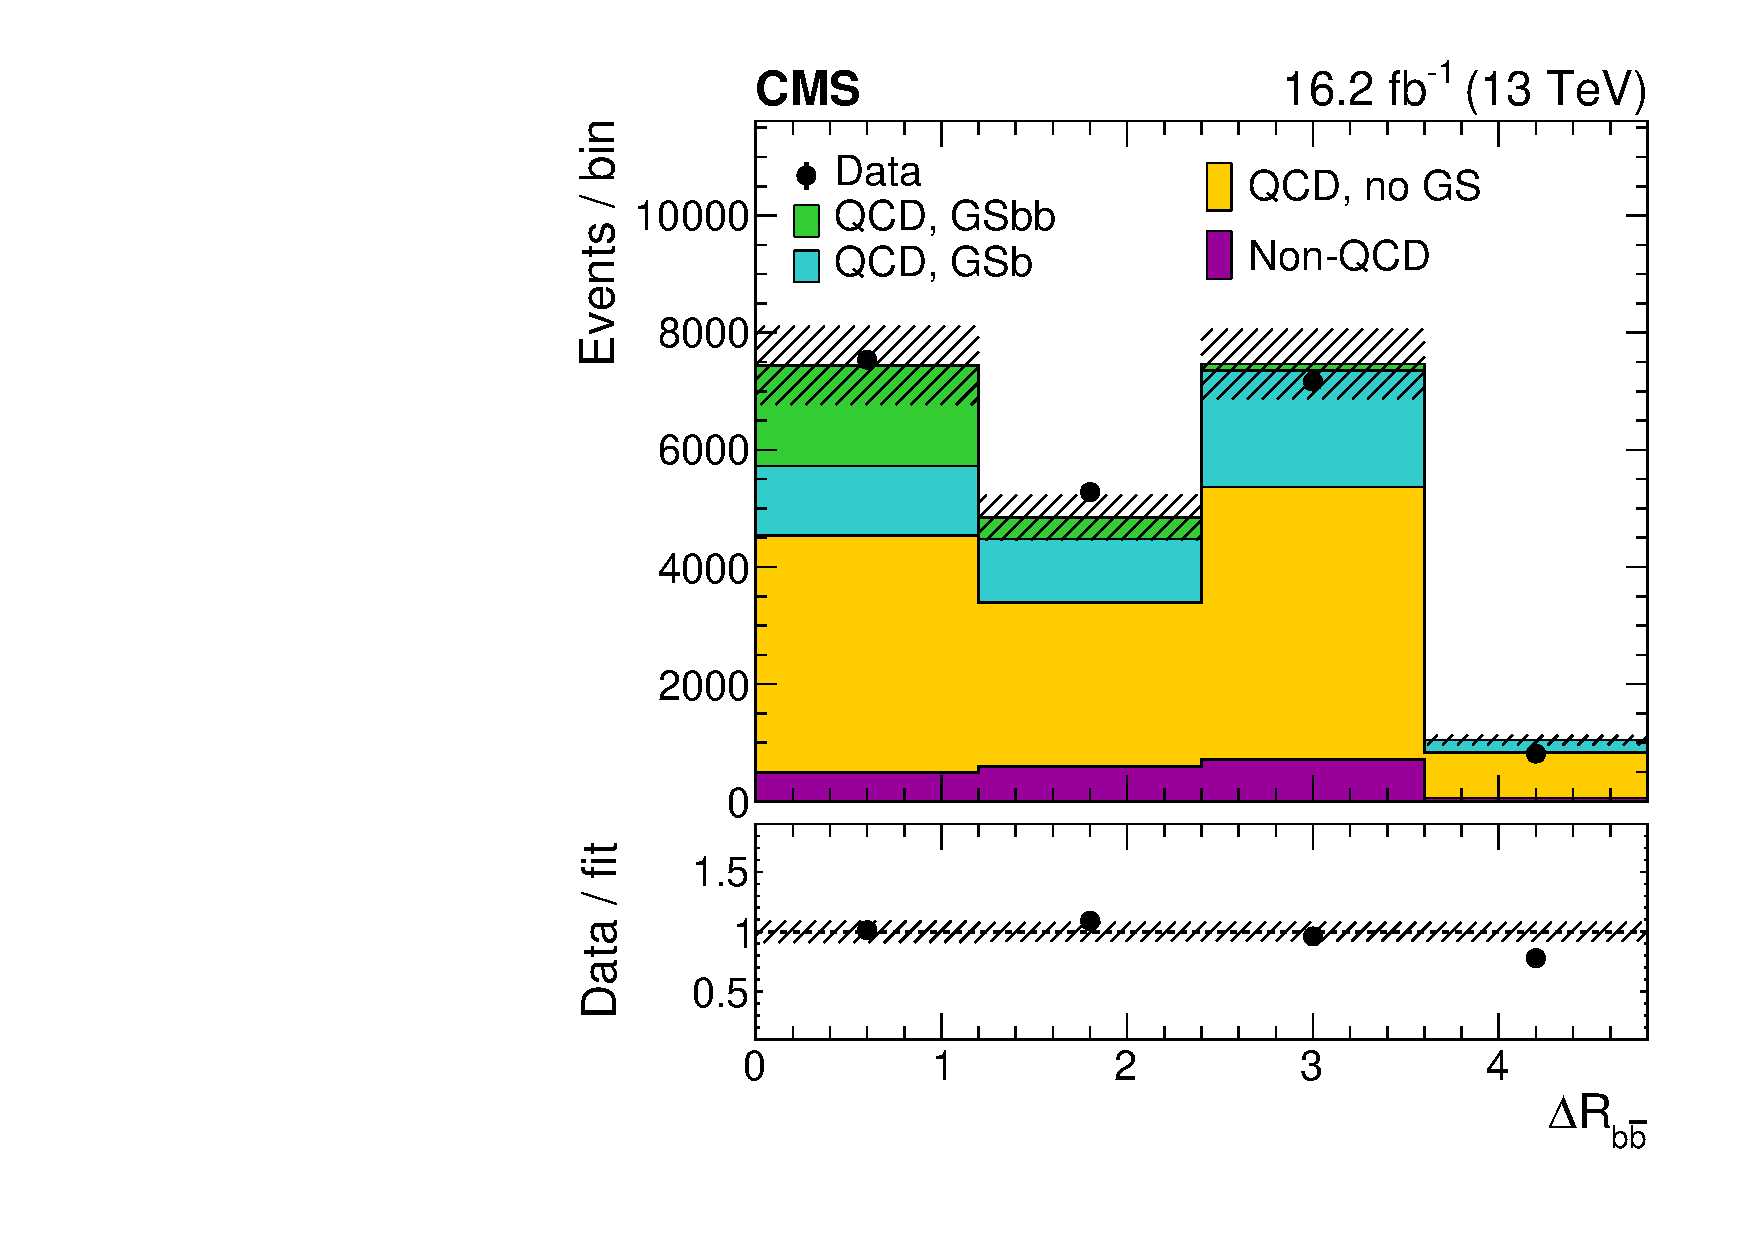
\includegraphics[angle=0,width=0.60\columnwidth]{fig/gs_fitresult.pdf}
\end{center}
\caption{Post-fit \dRbb distributions in a selection with  $\Nleps = 0$, $\HT > 1500~\GeV$, $\MJ > 500~\GeV$, $\Njets \geq 4$, and $\Nb = 2$ with the post-fit uncertainty represented by a hatched band.
The ratio of data to simulation yields is shown in the lower panel.}
\label{fig:gs_fitresult}
\end{figure}

\begin{figure}[tbp!]
\begin{center}
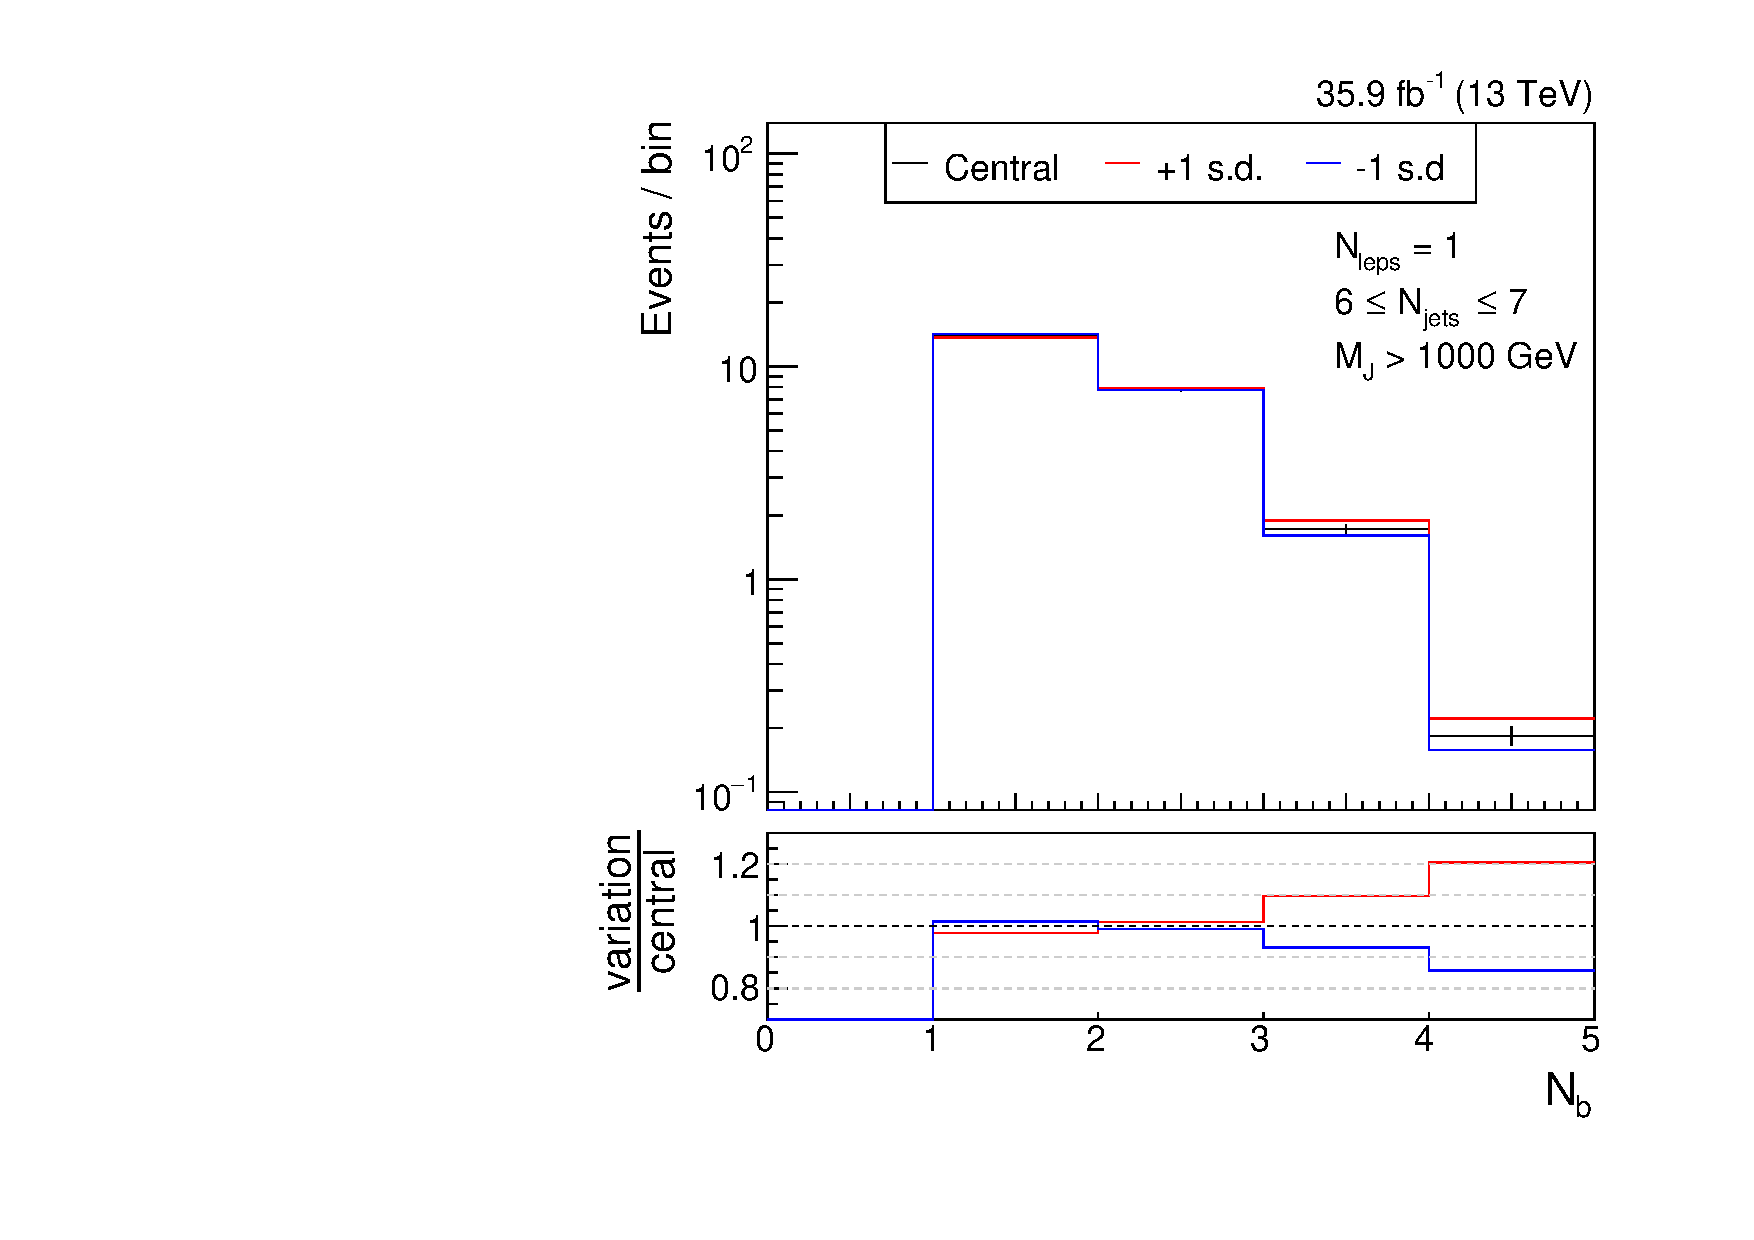
\includegraphics[angle=0,width=0.45\columnwidth]{fig/bin20_ttbar_gs_mconly.pdf}
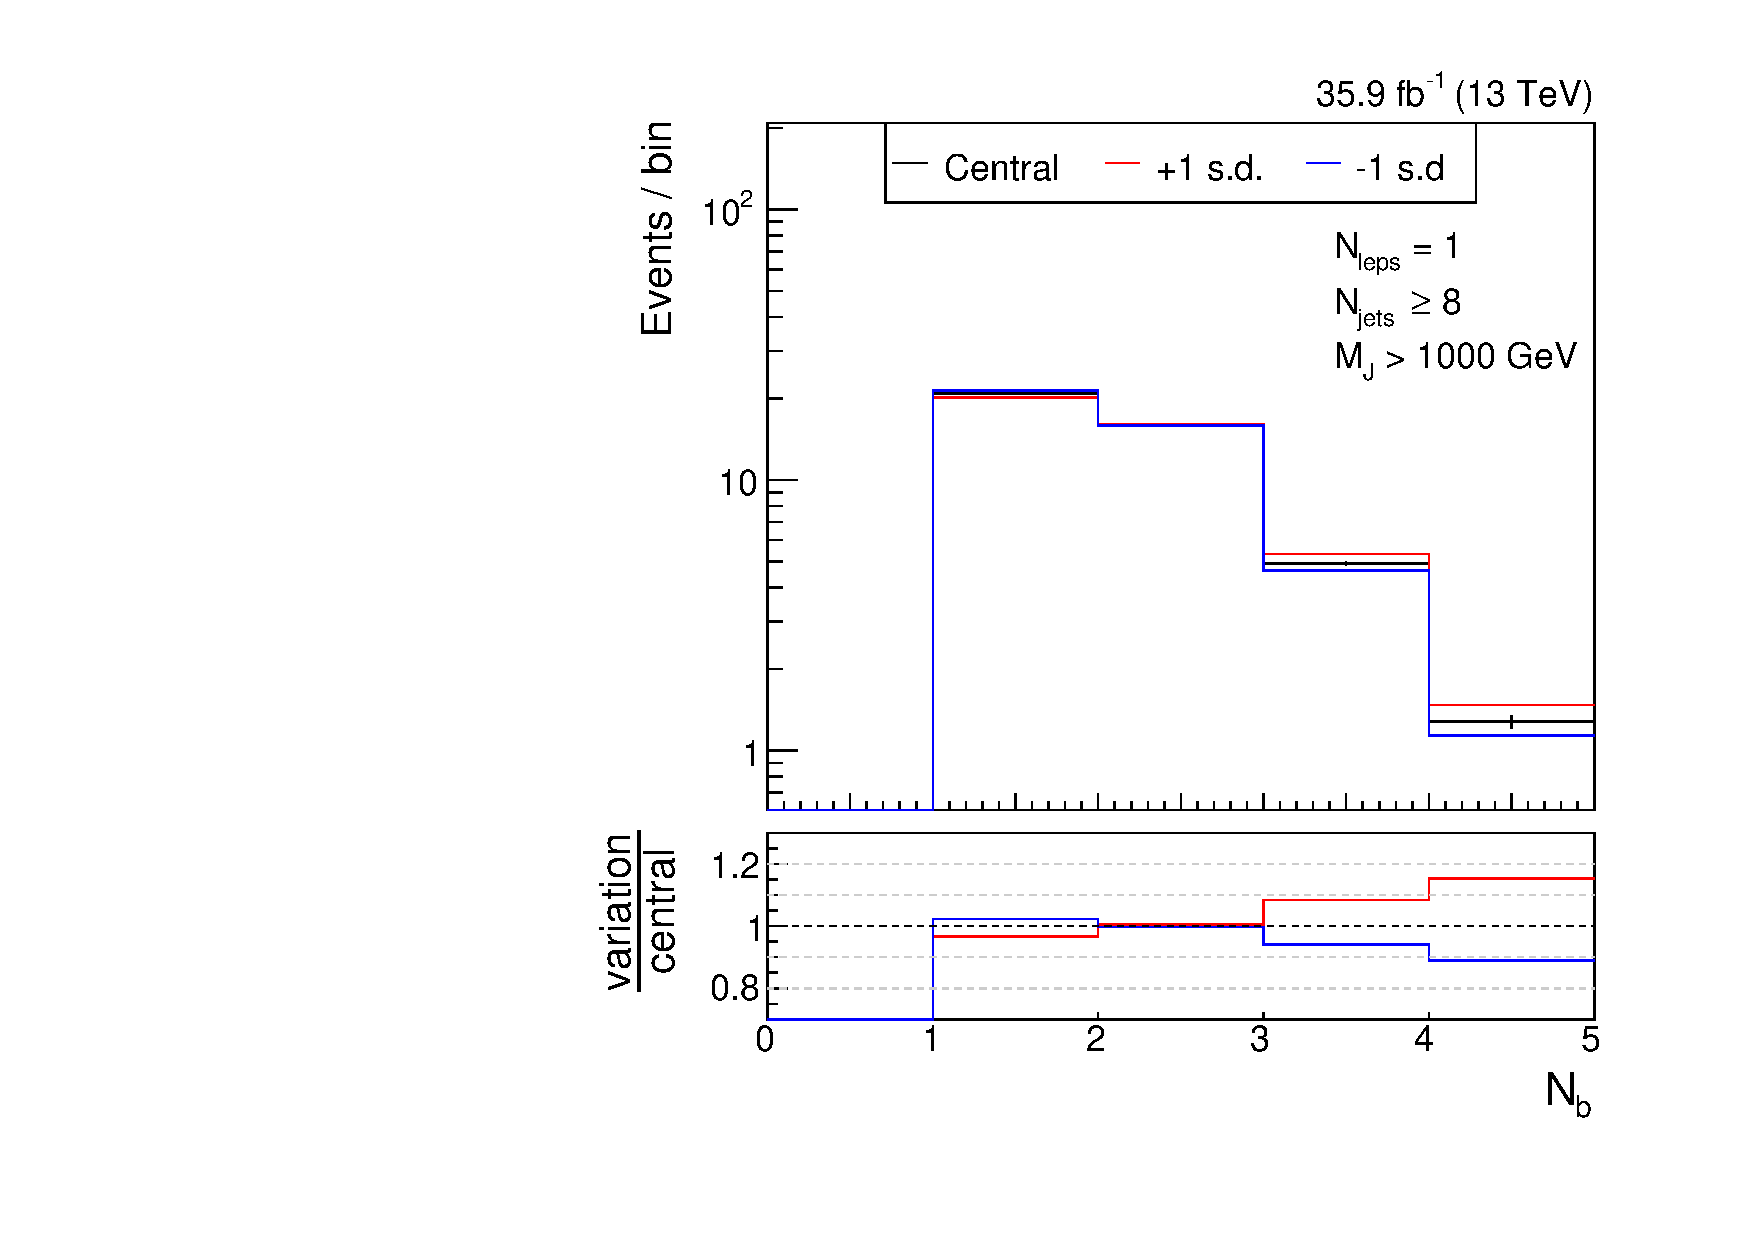
\includegraphics[angle=0,width=0.45\columnwidth]{fig/bin21_ttbar_gs_mconly.pdf}
\end{center}
\caption{Effect of the $\pm 1$~s.d.\ variations of the gluon splitting rate on the \Nb distribution in \ttbar normalized to $35.9~\ifb$ for the two most sensitive bins: ($\Njets \geq 8$, $800 < \MJ \leq 1000~\GeV$) (left) and ($\Njets \geq 8$, $\MJ > 1000~\GeV$) (right).}
\label{fig:gs_variations}
\end{figure}

In order to test the stability of the fit results and the dependence of the gluon splitting weights across kinematic regions, the \dRbb fit is repeated both with a higher \MJ threshold and with different \Njets bins. 
The resulting weights are shwon in Table~\ref{tab:gs_kinematic_bins} and are all consistent with those of the nominal fit.

\begin{table}[tb!]
\setlength\tabcolsep{3pt}
\centering
\begin{tabular}{l|cccccc}
 & Nominal & $\MJ > 800~\GeV$ & $4 \leq \Njets \leq 5$ & $6 \leq \Njets \leq 7$ & $8 \leq \Njets \leq 9$ & $\Njets \geq 10$ \\
\hline
GS    & $0.77 \pm 0.09$ & $0.70 \pm 0.38$ & $ 0.80 \pm 0.32$  & $ 0.76 \pm 0.14$ & $ 0.75 \pm 0.16$  & $ 0.95 \pm 0.36$ \\
No GS & $1.21 \pm 0.08$ & $1.28 \pm 0.35$ & $ 1.15 \pm 0.26$  & $ 1.22 \pm 0.13$ & $ 1.24 \pm 0.15$  & $ 1.05 \pm 0.36$ \\
\end{tabular}
\caption{Gluon splitting weights derived in the nominal fit, a variation with a requirement of $\MJ > 800~\GeV$, and 4 variations in bins of \Njets (with the nominal $\MJ > 500~\GeV$ requirement.)}
\label{tab:GS_variations}
\end{table}

\end{section}

\begin{section}{b-tagging Data-to-simulation Scale Factors}

Another significant systematic uncertainty is the uncertainty in the data-to-simulation scale factors (SF) for b~tagging efficiency and mistag rates.
These scale factors are derived from data in various QCD and \ttbar control samples and are binned in jet \pT and jet flavor (light + g, c, and b)~\cite{CMS-DP-2017-012}.
The $\pm 1$~s.d.\ \Nb templates for these scale factors are assessed by varying them according to the uncertainties in their measurements.
The effect of these variations on the \Nb distribution in \ttbar events is shown in Figure~\ref{fig:sf_variations}.

\end{section}

\begin{section}{Additional systematic uncertainties}

Other experimental uncertainties are small and include lepton selection efficiency, lepton misidentification rate, jet energy scale, jet energy resolution, and integrated luminosity.
The uncertainty associated with lepton selection efficiency is determined by varying the efficiency to select a lepton within its uncertainty determined from data.
The $\Nleps$ distribution for QCD events may not be simulated well because it relies on modeling the tail of the fragmentation function and various detector effects.
To account for this, an uncertainty of 20\% is assigned to the relative normalization of QCD events in the 0- and 1-lepton bins, which is motivated by data-to-simulation studies of lepton isolation distributions.
Jet energy scale uncertainties~\cite{Chatrchyan:2011ds,1748-0221-12-02-P02014} are assessed by varying the \pT of small-$R$ jets as a function of \pT and $\eta$.
The uncertainty arising from jet energy resolution~\cite{Chatrchyan:2011ds,1748-0221-12-02-P02014} is determined by applying an $|\eta|$-dependent factor to the jet \pT to match the jet energy resolution observed in data.
The integrated luminosity is varied according to its uncertainty of 2.5\%~\cite{CMS-PAS-LUM-17-001}, affecting only the backgrounds estimated from simulation.
No uncertainty is applied for the amount of pileup as studies have shown its effect to be negligible in this high-\HT selection.
The uncertainties due to the limited size of simulation samples are incorporated as uncorrelated nuisance parameters in the fit.

Theoretical systematic uncertainties are applied and include independent and correlated variations of the renormalization  and factorization scales.
Additionally, uncertainties on the PDF are incorporated by considering variations in the NNPDF 3.0 scheme~\cite{Ball:2014uwa}.
The size of these uncertainties is typically small as the effect of these variations is largely to modify the cross section of processes, which for the main backgrounds are constrained by data.

The background systematic uncertainties that affect the \Nb shape are shown in Figure~\ref{fig:bkg_sys_tables} for the two most sensitive search bin.

\begin{figure}[tbp!]
\begin{center}
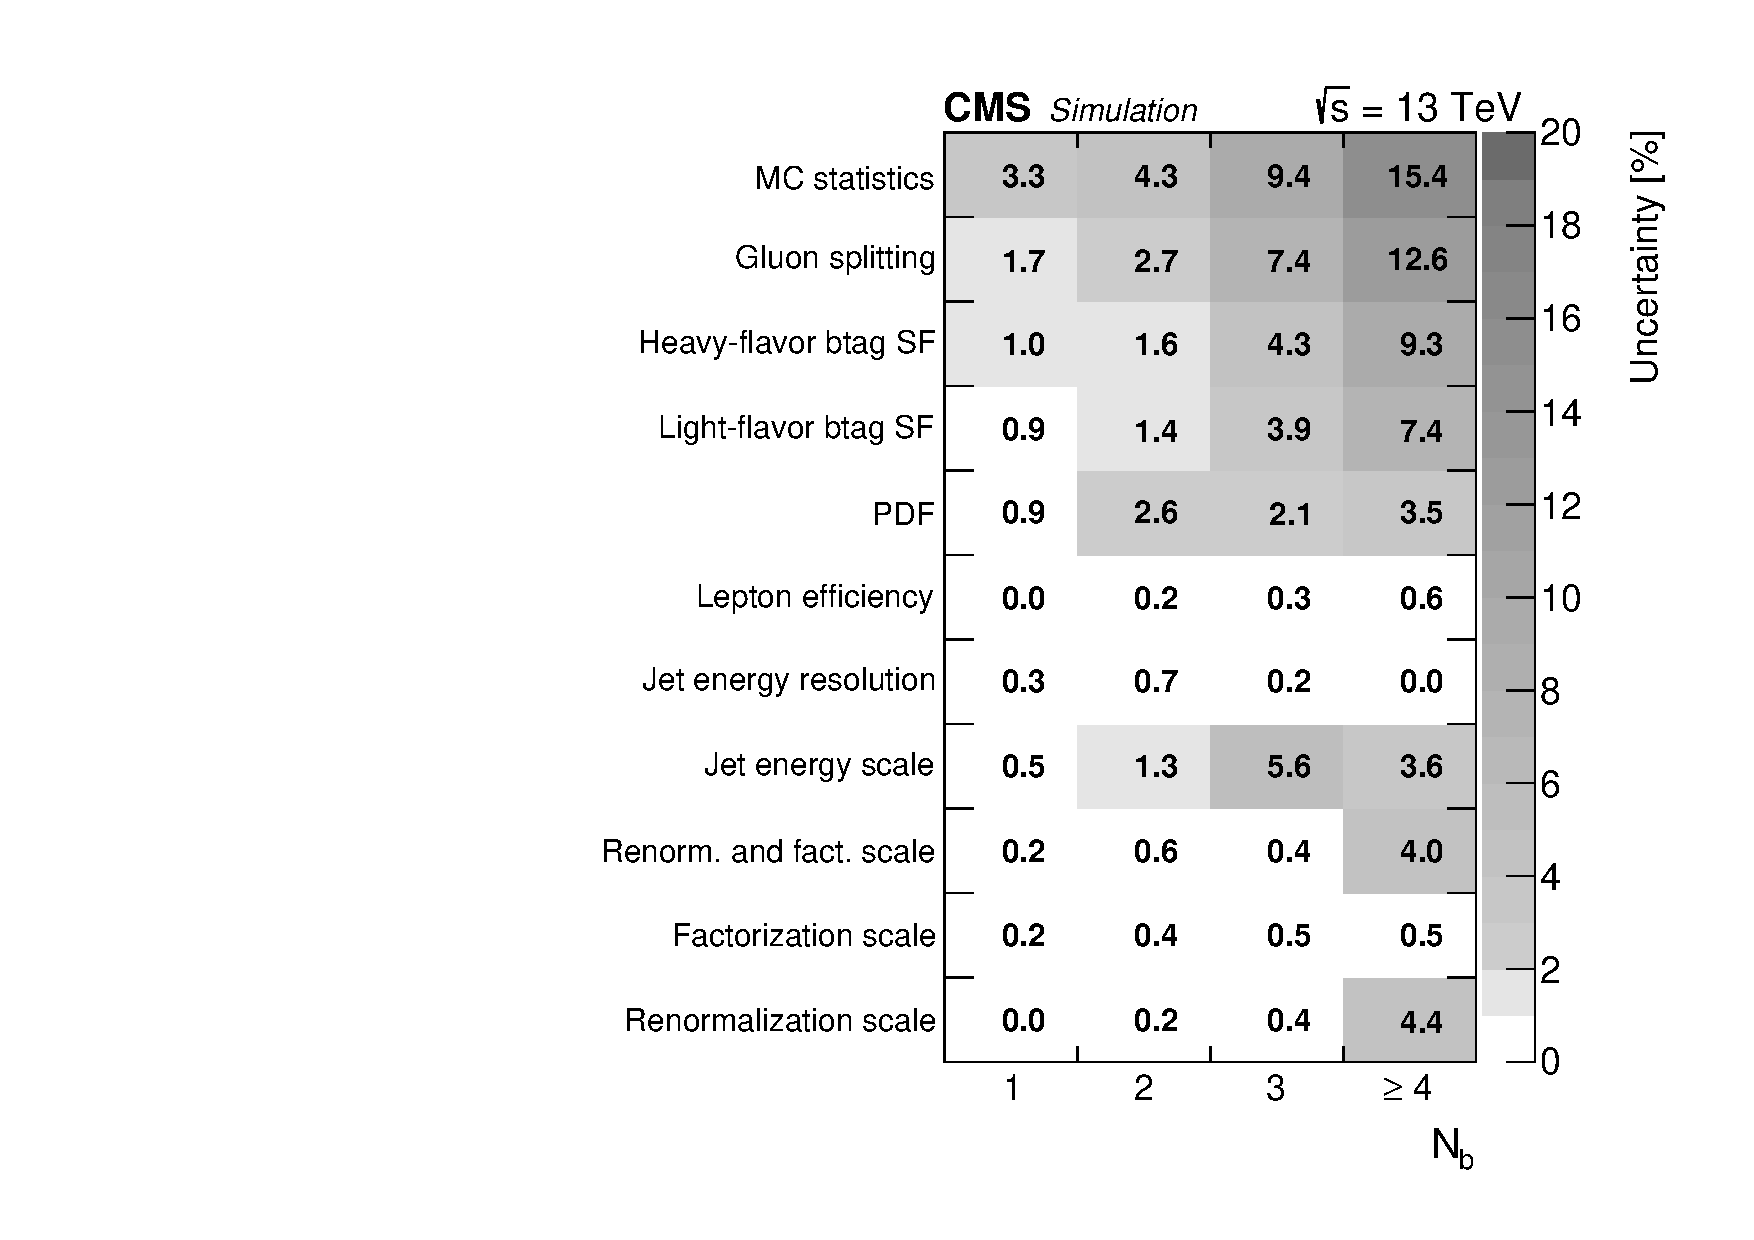
\includegraphics[angle=0,width=0.45\columnwidth]{fig/table_bkg_systs_bin20.pdf}
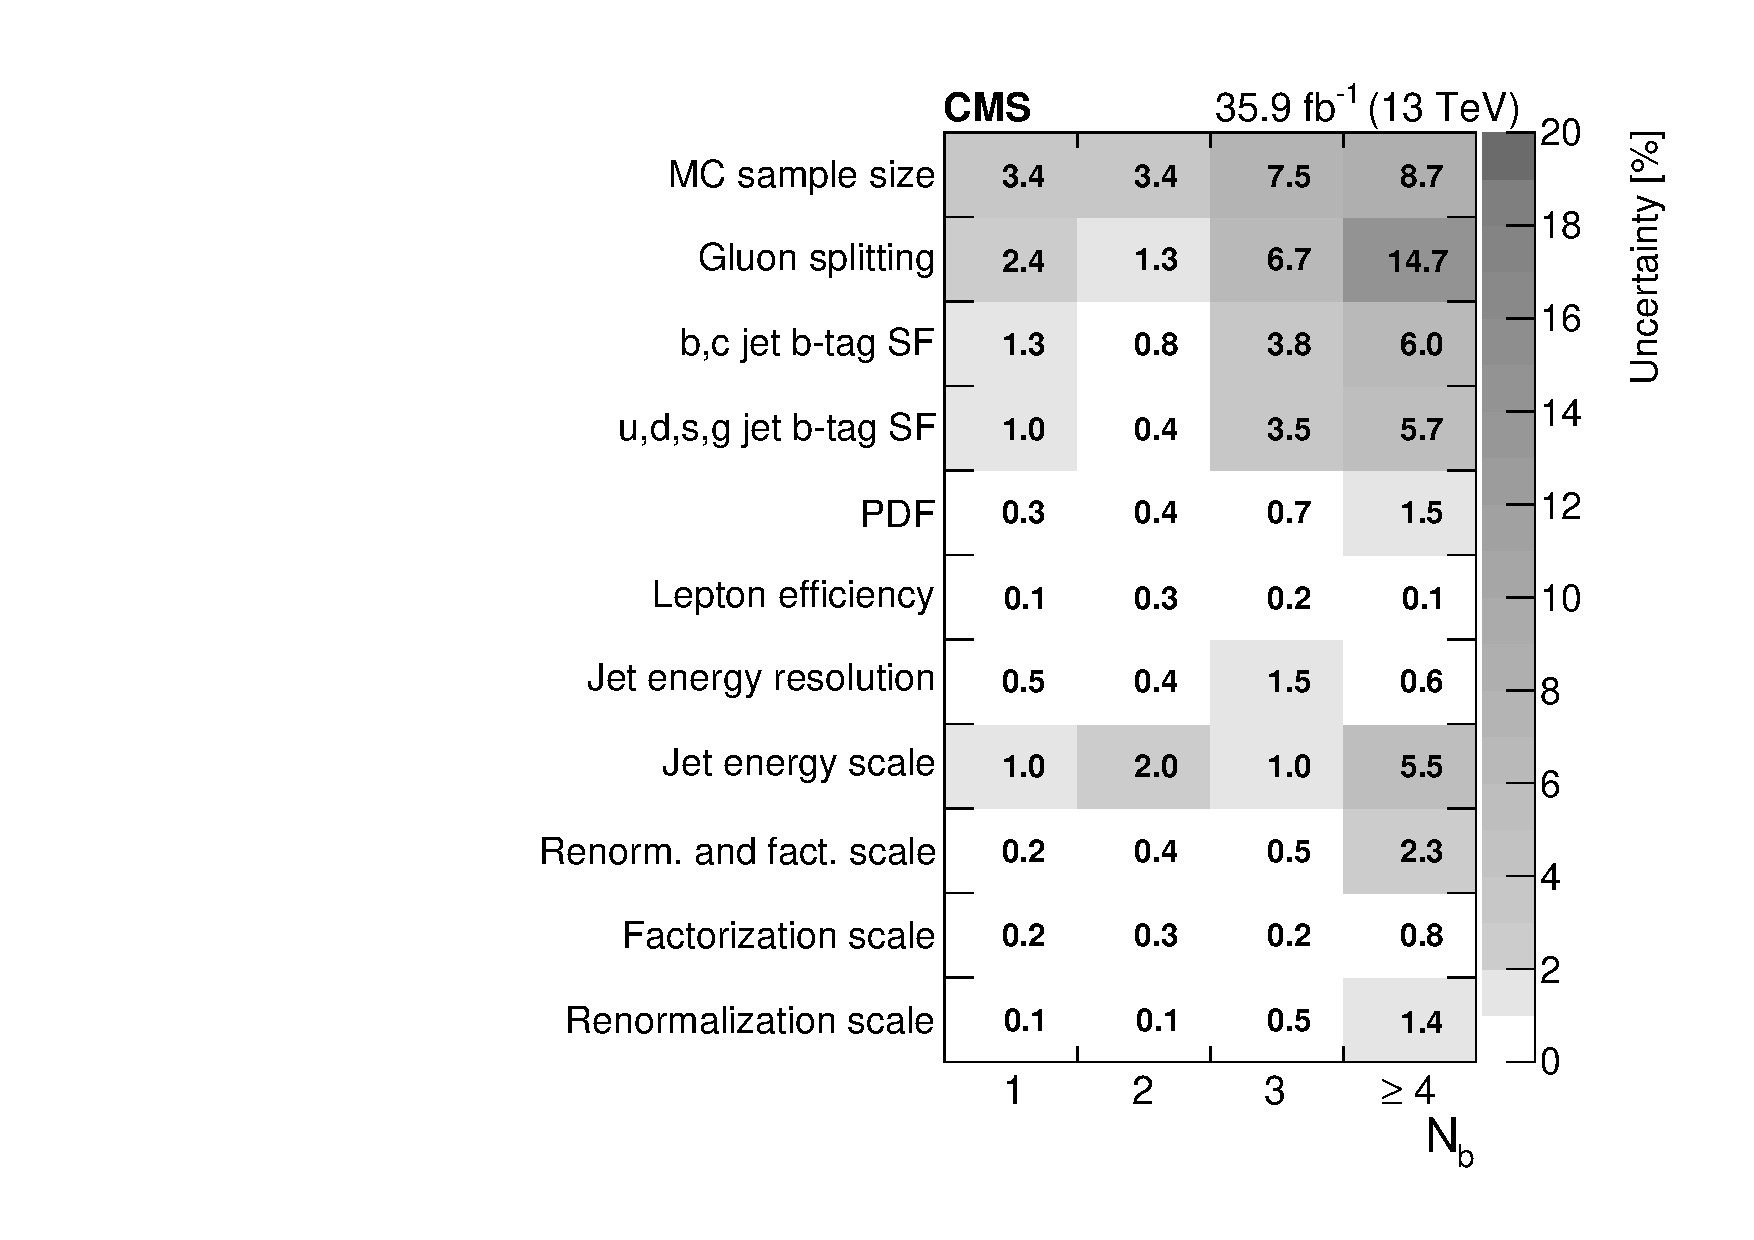
\includegraphics[angle=0,width=0.45\columnwidth]{fig/table_bkg_systs_bin21.pdf}
\end{center}
\caption{Background systematic uncertainties affecting the \Nb shape (in percent) for the ($\Njets \geq 8$, $500 < \MJ \leq 1000~\GeV$) (left) and ($\Njets \geq 8$, $\MJ > 1000~\GeV$) (right) bins.
The bottom row shows the total uncertainty for a given \Nb bin by summing in quadrature all uncertainties.
These values are similar for other (\Njets, \MJ) bins.}
\label{fig:bkg_sys_tables}
\end{figure}

\end{section}

\begin{section}{Signal Systematics}

Several of the systematic uncertainties affecting the signal yield are evaluated in the same way as the background yield.
These are the uncertainties due to gluon splitting, lepton selection efficiency, jet energy scale, jet energy resolution, b~tagging scale factors, simulation sample size, integrated luminosity, and theoretical uncertainties.
All systematic variations affect both the \Nb shape and normalization, except for the gluon splitting uncertainty, which is taken to affect only the \Nb shape.

The number of jets from ISR produced in the signal simulation is reweighted based on comparisons between data and simulated \ttbar samples.
The reweighting factors vary between 0.92 and 0.51 for the number of ISR jets between 1 and $\ge6$.
One half of the deviation from unity is taken as the systematic uncertainty in these reweighting factors.

The systematic uncertainties affecting the signal \Nb shape are shown in Fig.~\ref{fig:sig_sys_tables} (right) for the most sensitive bin in a model with $m_{\glu} = 1600~\GeV$.
The dominant signal systematic uncertainties arise from the limited simulation sample size, the b~tagging efficiency scale factors, and the ISR modeling.
There is no systematic uncertainty taken for pileup reweighting, as the signal efficiency is found to be insensitive to the number of pileup interactions, which is shown in Table~\ref{tab:sig_pu_dependence}.

\begin{figure}[tbp!]
\begin{center}
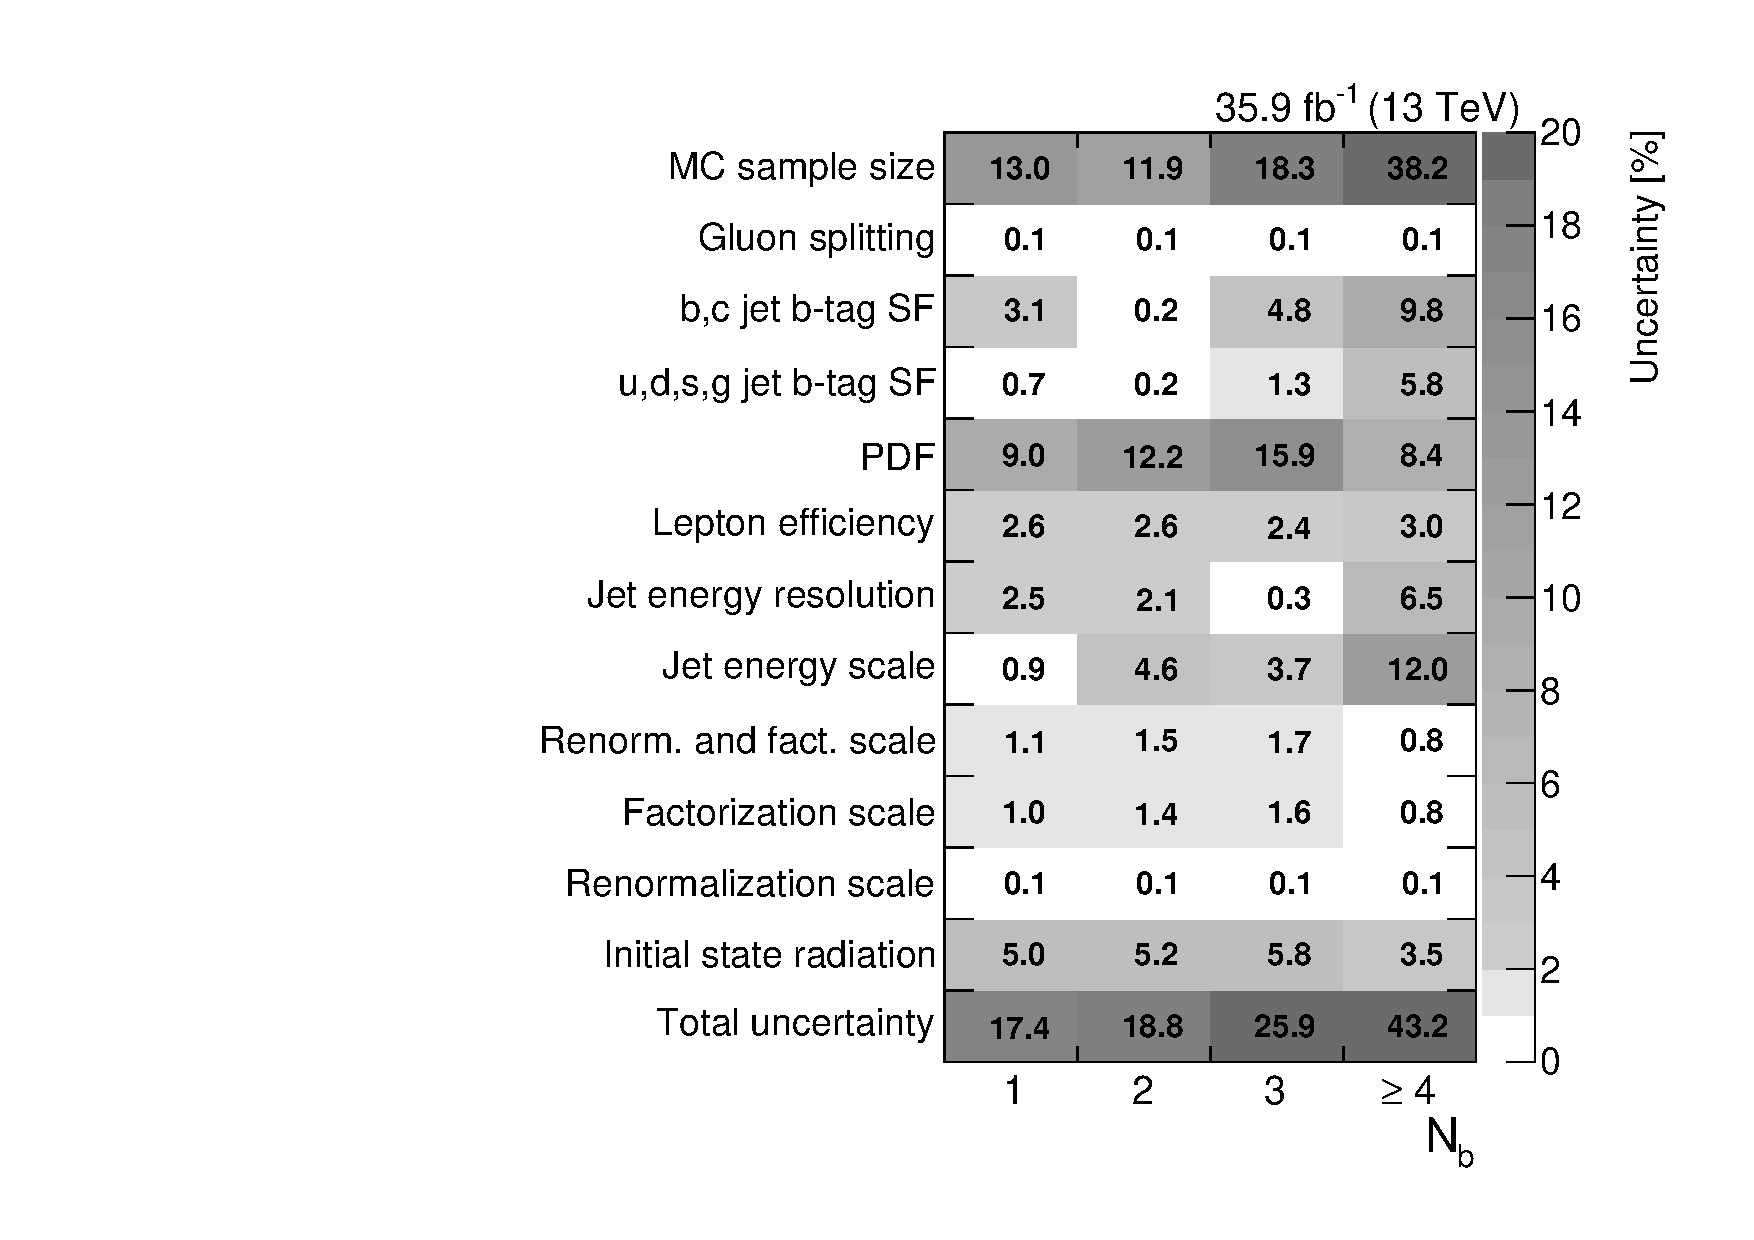
\includegraphics[angle=0,width=0.45\columnwidth]{fig/table_sig_systs_bin20_m1600.pdf}
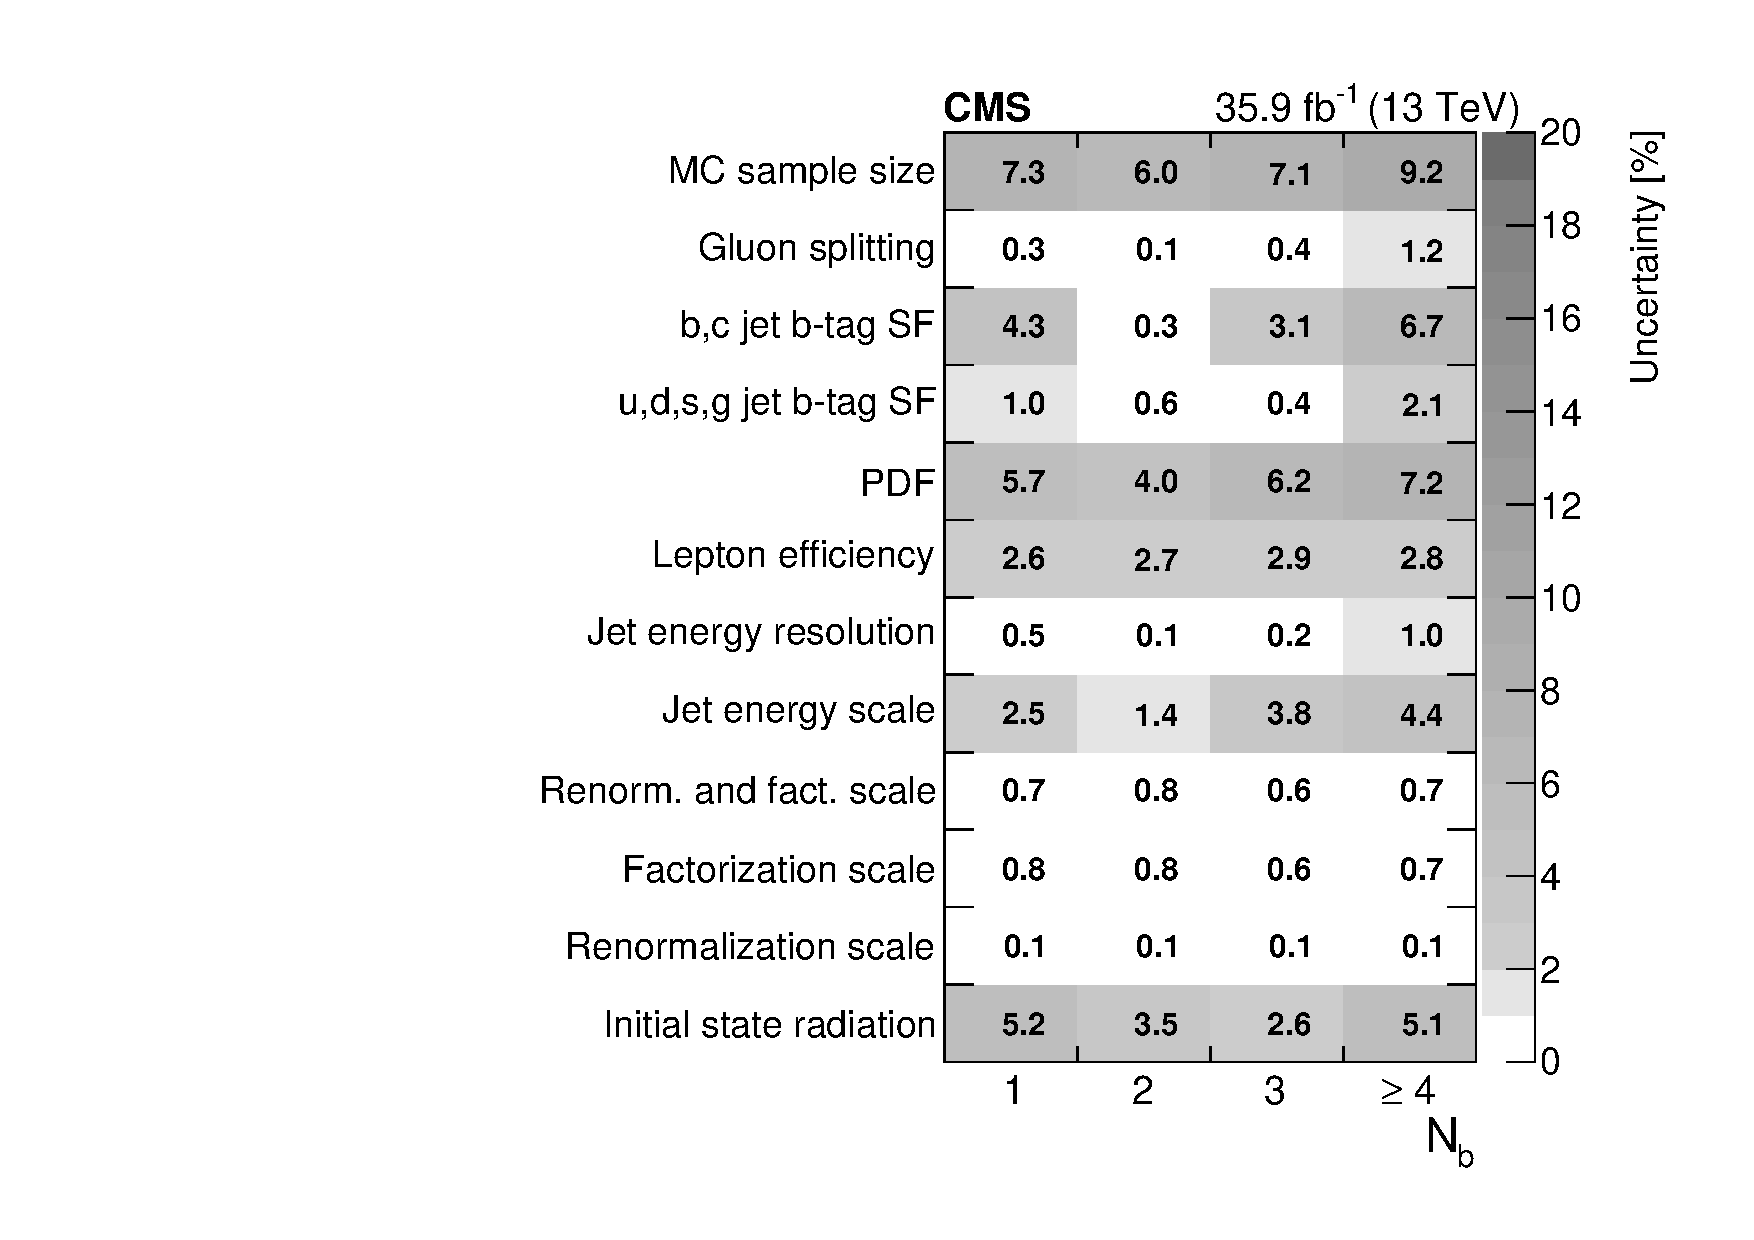
\includegraphics[angle=0,width=0.45\columnwidth]{fig/table_sig_systs_bin21_m1600.pdf}
\end{center}
\caption{Signal systematic uncertainties affecting the \Nb shape (in percent) for the ($\Njets \geq 8$, $500 < \MJ \leq 1000~\GeV$) (left) and ($\Njets \geq 8$, $\MJ > 1000~\GeV$) (right) bins.
The bottom row shows the total uncertainty for a given \Nb bin by summing in quadrature all uncertainties.
These values are similar for other (\Njets, \MJ) bins.}
\label{fig:sig_sys_tables}
\end{figure}

\begin{table}[tbp!]
\centering
\begin{tabular}{ |c|c|c| }
\hline
$N_{PV}^{true} \leq 20$ & $20 < N_{PV}^{true} \leq 40$ & $N_{PV}^{true} > 40$ \\ \hline
$8.0 \pm 0.5\%$ & $8.1 \pm 0.4\%$ & $7.5 \pm 1.5\%$ \\ \hline
\end{tabular}
\caption{The signal efficiency of the most sensitive bin ($\Njets \geq 8$, $\MJ > 1000~\GeV$) for a 1600~\GeV gluino in various bins of the number of truth-level primary vertices.}
\label{tab:sig_pu_dependence}
\end{table}

\end{section}

%TO DO
% 1. Check plot aesthetics since taken from AN, e.g. Preliminary -> Simulation
% 2. Gluon splitting shape plot with better range. (Check analysis/CWR comments or early version of paper).
% 3. Are categories GS -> qq -> 2 b-tagged jets or GS -> bb -> 2 b-tagged jets, etc
% 4. Add finer binned gs fit results plot.
% 5. Add plots for b-tag SF variation in ttbar
% 6. Expand ``other systematics'' section by going into detail about the lepton fake rate.
% 7. Use updated table for bkg sys that has the total uncertainty row.
% 8. Expand insensitivity on the pileup dependence with CWR explanation of why it doesn't matter.
% 9. Expand SF systematic section by discussing the Run split SFs.
% 10. Define \dR if not defined earlier in the document.
